
\documentclass[a4paper,11pt]{article}

% Math symbols
\usepackage{amsmath}
\usepackage{amsfonts}
\usepackage{esvect}
\usepackage{mhchem}

% Hyperlink contents page
\usepackage{hyperref}
\hypersetup{
	colorlinks,
	citecolor=black,
	filecolor=black,
	linkcolor=black,
	urlcolor=black
}

% No indent on new paragraphs
\setlength{\parindent}{0mm}
\setlength{\parskip}{0.2cm}

% AI files
\usepackage{graphicx}
\DeclareGraphicsRule{.ai}{pdf}{.ai}{}


\begin{document}

\title{Equilibrium}
\author{Ben Anderson}
\date{\today}
\maketitle
\pagebreak

\tableofcontents
\pagebreak



\section{Energy}

\subsection{Enthalpy}

Symbol: $H$

Units: $J$ (Joules)

Another term for energy.


\subsection{Change in Enthalpy}

Symbol: $\Delta H$

The amount of energy absorbed by or released into the surroundings over the
course of a chemical reaction.


\subsection{Activation Energy}

Energy required to start a reaction.

Reactions with low activation energy occur spontaneously.


\subsection{Energy Profile Diagrams}

A graph of enthalpy (in kJ) against the reaction coordinate (time).

Features on the graph include:

\begin{itemize}
\item Enthalpy of reactants and products
\item $\Delta H$
\item Activation energy for the forward and reverse reactions
\item Transition state (or activated complex)
\end{itemize}


\subsection{Exothermic}

A reaction that releases energy into its surroundings.

Increases temperature of surroundings.

$\Delta H < 0$

For example:

\begin{itemize}
\item Bond formation
\item Cellular respiration
\item Combustion
\item Condensation
\item Freezing
\item Formation of a precipitate
\end{itemize}

An exothermic energy profile diagram is shown in Figure \ref{fig:exothermic}.

\begin{center}
\begin{figure}
\resizebox{0.8\linewidth}{!}{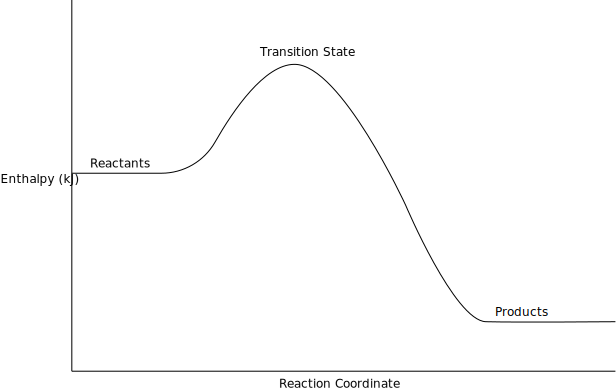
\includegraphics{exothermic.ai}}
\caption{An exothermic energy profile diagram}
\label{fig:exothermic}
\end{figure}
\end{center}


\subsection{Endothermic}

A reaction that absorbs energy from its surroundings.

Decreases the temperature of surroundings.

$\Delta H > 0$

For example:

\begin{itemize}
\item Bond breakage
\item Photosynthesis
\item Melting
\item Evaporation
\end{itemize}

An endothermic energy profile diagram is shown in Figure \ref{fig:endothermic}.

\begin{figure}
\begin{center}
\resizebox{0.8\linewidth}{!}{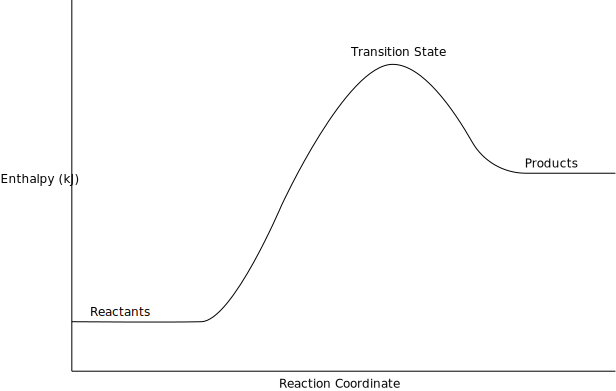
\includegraphics{endothermic.ai}}
\caption{An endothermic energy profile diagram}
\label{fig:endothermic}
\end{center}
\end{figure}




\section{Kinetic Theory}

\subsection{Reactions}

For a reaction to occur:

\begin{enumerate}
\item Particles must collide
\item With sufficient energy (greater than the activation energy)
\item In the correct orientation
\end{enumerate}


\subsection{Energy Distribution Diagram}

\begin{figure}
\begin{center}
\resizebox{0.8\linewidth}{!}{\includegraphics{distribution.ai}}
\caption{A sample energy distribution diagram}
\label{fig:distribution}
\end{center}
\end{figure}

An energy distribution diagram shows the number of particles with a particular
energy.


\subsection{Rate of Reaction}

The rate at which a reaction proceeds depends on two factors:

\begin{enumerate}
\item Frequency of collisions between particles.
\item Proportion of particles with energy greater than the activation energy.
\end{enumerate}


\subsubsection{Concentration}

Only applies to aqueous ions in solution.

Increasing the concentration of a species in solution increases the frequency
of collisions, increasing rate of reaction.


\subsubsection{Partial Pressure}

Only applies to gases.

Increasing the partial pressure of a species in a homogenous gas increases the
frequency of collisions, increasing rate of reaction.


\subsubsection{Surface Area}

Only applies to solids.

Increasing the surface area of a solid increases the frequency of collisions,
increasing rate of reaction.


\subsubsection{Temperature}

\begin{figure}
\begin{center}
\resizebox{0.8\linewidth}{!}{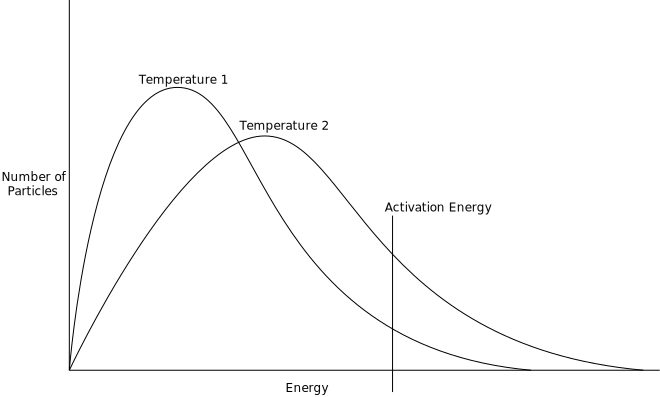
\includegraphics{temperature-distribution.ai}}
\caption{The energy distribution of particles when the temperature is increased}
\label{fig:temperature-distribution}
\end{center}
\end{figure}

Increasing the temperature increases the kinetic energy of the particles:

\begin{itemize}
\item Causes them to collide more frequently
\item Causes a greater proportion to have sufficient energy to react
\end{itemize}

The energy distribution diagram for particles when the temperature is increased
is shown in Figure \label{fig:temperature-distribution}. The peak moves down
and to the right.


\subsubsection{Catalyst}

A catalyst provides an alternate reaction pathway with a lower activation
energy.

Decreasing the activation energy increases the proportion of particles with
sufficient energy to react, increasing the rate of reaction.

A reaction profile diagram for a reaction with an added catalyst is shown in
Figure \ref{fig:catalyst-reaction}.

\begin{figure}
\begin{center}
\resizebox{0.8\linewidth}{!}{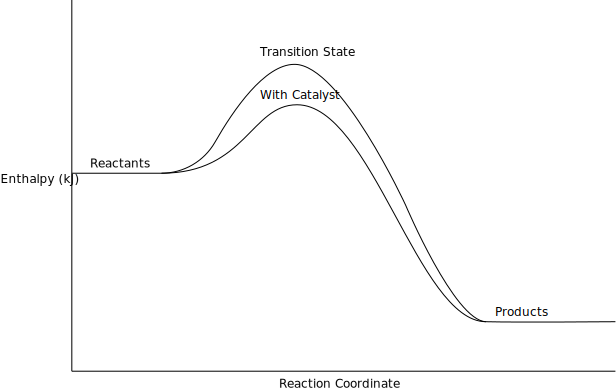
\includegraphics{exothermic-catalyst.ai}}
\caption{A reaction profile diagram for a reaction with a catalyst}
\label{fig:catalyst-reaction}
\end{center}
\end{figure}

An energy distribution diagram for a reaction with a catalyst is shown in
Figure \ref{fig:catalyst-distribution}.

\begin{figure}
\begin{center}
\resizebox{0.8\linewidth}{!}{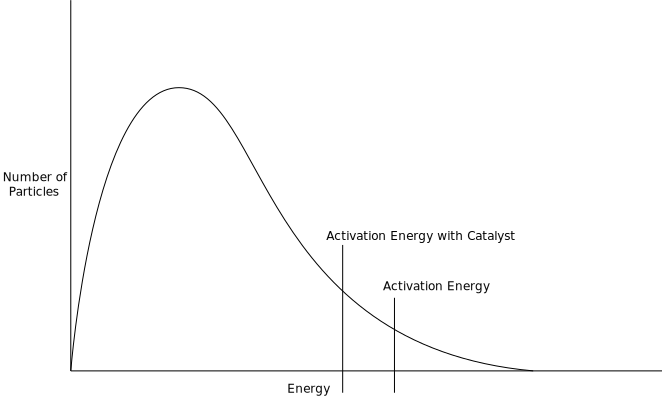
\includegraphics{catalyst-distribution.ai}}
\caption{An energy profile diagram for a reaction with a catalyst}
\label{fig:catalyst-distribution}
\end{center}
\end{figure}




\section{Equilibrium}

Exists for reversible reactions only.

A system is in equilibrium when the rate of the forward reaction equals the
rate of the reverse reaction.


\subsection{Physical Equilibrium}

For physical processes.

A solution is saturated when rate of dissolving of a solid equals the rate of
condensation.

Vapor pressure is when the rate of evaporation of a liquid equals the rate of
condensation.


\subsection{Chemical Equilibrium}

For a reversible chemical reaction.

For example:

$$
\ce{H2 (g) + I2 (g) <=> 2HI (g)}
$$

The system is in equilibrium when the rate of formation of $\ce{HI}$ (ie. the
rate of the forward reaction) equals the rate of formation of $\ce{H2}$ and
$\ce{I2}$ (ie. the rate of the reverse reaction).


\subsection{Rate vs. Time Graphs}

\begin{figure}
\begin{center}
\resizebox{0.8\linewidth}{!}{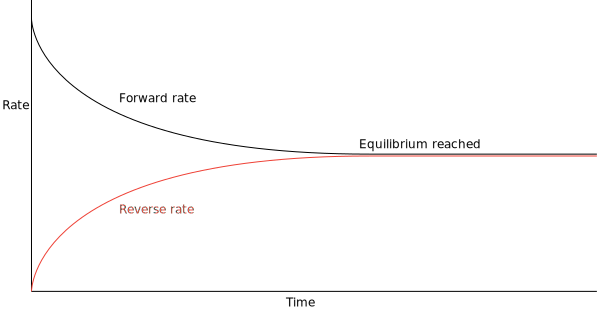
\includegraphics{equilibrium-rate.ai}}
\caption{Rate vs. time graph}
\end{center}
\end{figure}

Graph that show the relative rates of the forward and reverse reaction of an
equilibrium over time.

Initially:

\begin{itemize}
\item Forward reaction rate is high, as the concentration of reactants is high,
	causing a high frequency of collisions.
\item Reverse reaction rate is 0, as the concentration of products is 0.
\end{itemize}

Over time:

\begin{itemize}
\item Reverse rate increases as the concentration of products increases due to
	the forward reaction.
\item Forward rate decreases, as concentration of reactants decreases due to
	the forward reaction producing more products.
\end{itemize}

Equilibrium is established when the forward rate equals the reverse rate.


\subsection{Concentration vs. Time Graphs}

Graph that shows the relative concentrations of all reactants and products of
an equilibrium over time.

Initially:

\begin{itemize}
\item Concentration of reactants is high.
\item Concentration of products is 0.
\end{itemize}

After equilibrium has been established:

\begin{itemize}
\item Concentration of reactants has decreased.
\item Concentration of products has increased.
\item Concentration changes according to the stoichiometric ratios given in the
	equation for the equilibrium.
\end{itemize}

For the reaction:

$$
\ce{H2 (g) + I2 (g) <=> HI (g)}
$$

A concentration vs. time graph is shown in Figure
\ref{fig:equilibrium-concentration}.

\begin{figure}
\begin{center}
\resizebox{0.8\linewidth}{!}{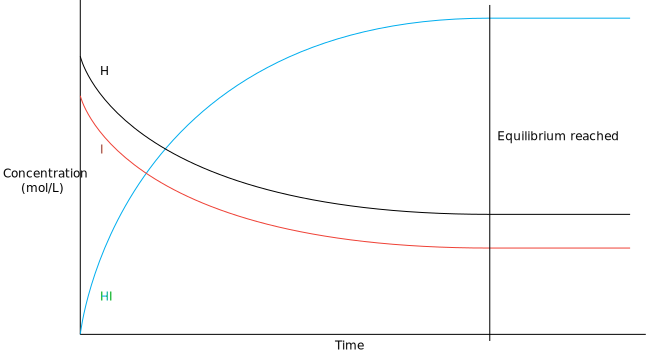
\includegraphics{equilibrium-concentration.ai}}
\caption{Concentration vs. time graph}
\label{fig:equilibrium-concentration}
\end{center}
\end{figure}


\subsection{Equilibrium Constant}

The equilibrium constant is a value that represents the relative concentrations
of the reactants and products in a system when it is in equilibrium.

For the equation:

$$
\ce{aA + bB <=> cC + dD}
$$

The equilibrium constant is:

$$
E_K = \frac{[\mbox{C}]^c [\mbox{D}]^d}{[\mbox{A}]^a [\mbox{B}]^b}
$$

Ignore solids and liquids (eg. $\ce{H2O}$) when calculating the constant.


\subsubsection{Temperature}

The equilibrium constant remains constant for a given temperature.

Any imposed change on the system, apart from changing the temperature, will not
change the equilibrium constant.


\subsubsection{Concentrations}

The equilibrium constant can tell us the relative concentrations of the
reactants and products.

If $E_k > 1$, then the concentration of products is greater than reactants.
The equilibrium lies to the right.

If $E_k < 1$, then the concentration of reactants is greater than products.
The equilibrium lies to the left.


\subsection{Equilibrium Position}

The equilibrium position refers to the relative concentrations of reactants and
products for the equilibrium constant.

When the equilibrium shifts left, the concentration of the reactants increases,
and products decreases. Favours the reverse reaction.

When the equilibrium shifts right, the concentration of the products increases,
and reactants decreases. Favours the forward reaction.

Only changes to substances included in the equilibrium constant calculation will
affect the position of the equilibrium. Solids and liquids do not have an
effect.


\subsection{Le Chatelier's Principle}

When a change is imposed on a system in equilibrium, the equilibrium position
will shift to partially counteract the change.


\subsection{Concentration}

Changes to the concentration of one species must be explained using collision
theory.

Increase in concentration of a reactant:

\begin{itemize}
\item Immediately increases frequency of collisions between reactants,
	increasing rate of forward reaction.
\item Increases concentration of products over time.
\item Increases frequency of collisions between products, increasing reverse
	rate over time.
\item Concentration of reactants decreases as more products are formed,
	decreasing rate of forward reaction over time.
\end{itemize}

Decrease in concentration of a reactant:

\begin{itemize}
\item Immediately decrease frequency of collisions between reactants, decreasing
	rate of forward reaction.
\item The relatively higher rate of the reverse reaction at this instant
	increases the concentration of the reactants over time, increasing the
	forward rate over time.
\item The reduced forward rate decreases the concentration of the products
	over time.
\item Decreases frequency of collisions between products, decreasing reverse
	rate over time.
\end{itemize}


\subsubsection{Rate vs. Time Graph}

At the instant the concentration of a reactant is increased:

\begin{itemize}
\item Immediate increase in forward rate.
\item Gradual decrease of forward rate over time.
\item Gradual increase in reverse rate over time.
\end{itemize}


\subsubsection{Concentration vs. Time Graph}

At the instant the concentration of a reactant is increased:

\begin{itemize}
\item Immediate increase in concentration of reactant that is added.
\item Gradual decrease in reactant over time, finishing just above where it
	started.
\item Gradual decrease in concentration of other reactants.
\item Gradual increase in concentration of products.
\item Changes in concentration will conform to stoichiometric ratios in
	equation.
\end{itemize}


\subsubsection{Ways to Change Concentration}

\begin{itemize}
\item Adding an acid or base to react $\ce{H+}$ or $\ce{OH-}$ ions in the
	equation, including $\ce{NH3}$ as a base.
\item Forming an insoluble precipitate.
\end{itemize}


\subsection{Total Concentration}

Adding water to an equilibrium in a solution will decrease the concentration
of all species.

Le Chatelier's Principle states that the system will attempt to counteract this
change by shifting the equilibrium towards the side with more particles to
increase total concentration of all ions.

Identical to a change in total pressure for a gaseous system.


\subsection{Partial Pressure}

Identical to concentration for a gaseous system.


\subsection{Total Pressure}

Increasing the total pressure of a system will increase the partial pressure of
all gases in the system.

Le Chatelier's Principle states that the system will attempt to offset this
change by shifting the equilibrium towards the side with the least particles
to reduce total pressure.

For example:

$$
\ce{Cl2 (g) + 3F2 (g) <=> 2ClF3 (g)}
$$

Increasing the total pressure will cause equilibrium to shift right, as only 2
moles of gas are produced, compared to 4 on the left.


\subsubsection{Rate vs. Time Graph}

The rate belonging to the side with the most moles of gas is always affected
the most.

For an increase in total pressure:

\begin{itemize}
\item Both rates will increase immediately.
\item The rate belonging to the side of the equilibrium with more moles will
	increase more, and decrease over time.
\item The other rate will increase over time.
\end{itemize}

For a decrease in total pressure:

\begin{itemize}
\item Both rates will decrease immediately.
\item The rate belonging to the side of the equilibrium with the most moles of
	gas will decrease the most and increase over time.
\item The other rate will decrease over time.
\end{itemize}


\subsubsection{Concentration vs. Time Graph}

For an increase in total pressure:

\begin{itemize}
\item Concentration of all reactants and products increases immediately in
	stoichiometric ratios. For example, in the equilibrium $\ce{2A <=> B}$, A
	will increase twice as much as B.
\item Concentration of the species belonging to the side with the most moles
	of gas will decrease over time in stoichiometric ratios.
\item Concentration of other species will increase over time in stoichiometric
	ratios.
\end{itemize}


\subsubsection{Ways of Changing Total Pressure}

\begin{itemize}
\item Change volume of container.
\item Add an inert gas at constant pressure and temperature (changing volume).
	Decreases the partial pressure of all reactants.
\item Add an inert gas at constant volume and temperature (changing pressure).
	Has no effect on equilibrium, as partial pressures remain constant.
\end{itemize}


\subsection{Temperature}

As the temperature is increased, the system will attempt to offset this change
by favouring the endothermic reaction.

As the temperature is decreased, the system will attempt to offset this change
by favouring the exothermic reaction.

Changes the equilibrium constant.


\subsubsection{Rate vs. Time Graph}

The endothermic reaction is always affected more.

For an increase in temperature:

\begin{itemize}
\item Both rates will increase immediately.
\item The endothermic rate will increase more, and will decrease over time.
\item The exothermic rate will increase over time.
\end{itemize}

For a decrease in temperature:

\begin{itemize}
\item Both rates will decrease immediately.
\item The endothermic rate will decrease more, and will increase over time.
\item The exothermic rate will decrease over time.
\end{itemize}


\subsubsection{Concentration vs. Time Graph}

For an increase in temperature:

\begin{itemize}
\item The products for the endothermic reaction will decrease in concentration
	over time.
\item The reactants for the endothermic reaction will increase in concentration
	over time.
\item Will change in stoichiometric ratios.
\end{itemize}


\subsection{Catalyst}

Both forward and reverse rates will increase immediately by the same amount
after the addition of a catalyst.

No change in concentration of any species.

Rate vs. time graph shows an immediate increase in both rates by the same
amount. The system remains in equilibrium.

Concentration vs. time graph shows no change.


\subsection{Optimal Conditions}

Chose a pressure and temperature combination for an equilibrium reaction which
results in a high rate of reaction and high yield.

For example:

$$
\ce{2A + B <=> C} \quad \Delta H > 0
$$

High temperature would favour the endothermic (forward) reaction, increasing
yield. Also increases frequency of collisions and proportion of particles with
sufficient energy to react, increasing rate of reaction.

High pressure would shift the equilibrium right, favouring the forward
reaction, increasing yield. Also increases frequency of collisions, increasing
rate of reaction.


\subsubsection{Conflicting Requirements}

Where a moderate temperature or pressure must be selected to satisfy conflicting
rate of reaction and high yield requirements.

For example:

$$
\ce{H2 (g) + 3N2 (g) <=> 2NH3 (g)} \quad \Delta H > 0
$$

For temperature:

\begin{itemize}
\item Require a high temperature for fast rate of reaction.
\item Require a low temperature to favour the endothermic (forward) reaction for
	high yield.
\item Thus require a moderate temperature to satsify conflicting requirements.
\end{itemize}

Similar conflicting requirements for pressure.




\section{Haber Process}

The production of ammonia gas:

$$
\ce{N2 (g) + 3H2 (g) <=> 2NH3 (g)} \quad \Delta H = -92\text{ kJ}
$$

$\ce{N2}$ filtered from the air.

$\ce{H2}$ produced through the steam reforming process.


\subsection{Conditions}

Require a moderate temperature of $350^\circ\text{ C}$ to $550^\circ\text{ C}$
to satisfy conflicting requirements.

Require high pressure of 10 - 25 MPa for high yield and rate of reaction.

$\ce{Fe3O4}$ as catalyst. Pass gases through it as a porous material.


\subsection{Yield}

20\% to 30\%.

Increase yield by separating unreacted $\ce{N2}$ and $\ce{H2}$ and reusing.


\subsection{Steam Reforming}

Produces $\ce{H2}$.


\subsubsection{Steam Reforming Reaction}

$$
\ce{CH4 (g) + H2O (g) <=> CO (g) + 3H2 (g)} \quad \Delta H = +206\mbox{ kJ}
$$

High temperature ($700^\circ\text{ C}$ to $1000^\circ\text{ C}$).

Compromise pressure (1 to 2 MPa)

Nickel catalyst.


\subsubsection{Shift Reaction}

$$
\ce{CO (g) + H2O (g) <=> CO2 (g) + H2 (g)} \quad \Delta H = -41\mbox{ kJ}
$$

High pressure (1 to 2 MPa).

Compromise temperature ($200^\circ\text{ C}$ to $500^\circ\text{ C}$)

Catalyst is mixture of $\ce{Fe2O4}$, $\ce{Cr2O}$, $\ce{CuO}$, $\ce{ZnO}$.




\section{Contact Process}

The production of sulfuric acid in two stages.

\subsection{Stage 1}

$$
\ce{2SO2 (g) + O2 (g) <=> 2SO3 (g)} \qquad \Delta H = -196\mbox{ kJ}
$$

High pressure (around 100 kPa).

Compromise temperature ($400^\circ\text{ C}$ to $500^\circ\text{ C}$)

$\ce{V2O5}$ as catalyst.


\subsection{Stage 2}

$$
\ce{H2SO4 (g) + SO3 (g) -> H2S2O7 (g)}
$$

$$
\ce{H2S2O7 (g) + H2O (g) -> H2SO4 (g)}
$$

$\ce{SO3}$ is fed into an absorption tower, meeting a counterflow of diluted
98\% $\ce{H2SO4}$.

Reacts to form $\ce{H2S2O7}$ (100\% $\ce{H2SO4}$) which is filtered out.

Some is diluted to 98\% and reused. Some is stored and sold.

Water is not used as the reaction between $\ce{SO3}$ and $\ce{H2O}$ is violently
exothermic. Forms a hot mist which takes a long time to cool and condense.
Container would explode from sudden pressure increase.




\section{Sample Questions}

\subsection{Question 1}

Explain the shape of a rate vs. time graph for an equilibrium.


\subsection{Question 2}

Explain the change to an equilibrium between aqueous ions in solution when water
is added.

Explain the shape of a rate vs. time and concentration vs. time graph when this
occurs.


\subsection{Question 3}

Explain the change to a gaseous equilibrium when an inert gas is added at a
fixed volume and temperature.

\begin{itemize}
\item No change to the equilibrium position as there is no change to the partial
	pressure of any of the gases.
\end{itemize}


\subsection{Question 4}

Explain the change to a gaseous equilibrium when an inert gas is added at a
fixed pressure and temperature.

Explain the shape of a rate vs. time and concentration vs. time graph when this
occurs.


\subsection{Question 5}

A saturated solution is prepared by dissolving excess solid in water (leaving
some undissolved solid remaining). Explain the effect on the equilibrium when
more solid is added, and when some of the excess solid is removed.


\subsection{Question 6}

Explain the shape of a rate vs. time graph for an equilibrium when the
concentration of one product is increased/decreased.


\subsection{Question 7}

Explain the shape of a rate vs. time graph for an equilibrium when the
temperature is increased/decreased.

\end{document}
